\documentclass[9pt,twocolumn,twoside]{styles/osajnl}
\usepackage{fancyvrb}
\journal{i524} 

\title{An Overview of Apache Sqoop}


\author[1,*]{Harshit Krishnakumar}

\affil[1]{School of Informatics and Computing, Bloomington, IN 47408, U.S.A.}
\affil[*]{Corresponding authors: harkrish@iu.edu, S17-IR-2014}

\dates{Project-01, \today}

\ociscodes{Cloud, I524}

% replace this with your url in github/gitlab
\doi{\url{https://github.com/harkrish1/sp17-i524/blob/master/paper1/S17-IR-2014/report.pdf}}


\begin{abstract}
Big Data is increasingly being used in conjunction with RDBMS systems to perform every day analyses. In light of these requirements, we need to have an efficient system to transfer data between RDMBS and Hadoop systems. Sqoop provides an interface to efficiently manage data movement activities between these systems. This paper describes the different components and the operation of Sqoop\newline
\end{abstract}

\setboolean{displaycopyright}{true}

\begin{document}

\maketitle

\section{Introduction}

Hadoop systems are known to efficiently store transactional or log data in distributed file systems, as opposed to the traditional RDBMS systems which store relatively smaller volumes of data in database tables. Often times we would need to combine the transaction logs with the RDBMS data to perform analyses. Sqoop is the method of transferring data between RDBMS and Hadoop systems. Often there will be multiple RDBMS sources to operate on, Sqoop helps in automating these tasks by providing specific connectors to Teradata, Netezza, Oracle, MySQL, Postgres, and HSQLDB. 

Sqoop also leverages the parallel processing capabilities of Hadoop to transfer data. Sqoop integrates with Oozie, allowing developers to schedule and automate import and export tasks. Sqoop uses a connector based architecture which supports plugins that provide connectivity to new external systems.

Sqoop supports daily incremental data loads, production workflows for division of roles and administrators and also supports different security compliances. The latest release of Sqoop provides a rest API and Java API for easy integration along with a Hue UI and a command line client.\cite{cloudera}

\section{High Level Architecture}

Figure \ref{fig:archi} shows the High Level Architecture of how Sqoop works. Sqoop keeps different clients separate so that none of them have access to the entire set data, or rather have access to a specific subset for security purposes. Each client sends requests to a common Sqoop server which acts as an interface between client face and the actual servers. When Sqoop receives multiple requests, it prioritizes and sends the requests. The next step is to get the metadata from tables in RDBMS and use MapReduce to split the job between nodes. Sqoop server does not actually handle any data, rather it is just an agent which handles the jobs or requests. The data flows between Hadoop and RDBMS servers as instructed by Sqoop server\cite{sqoop-blog}.

\begin{figure}[htbp]
\centering
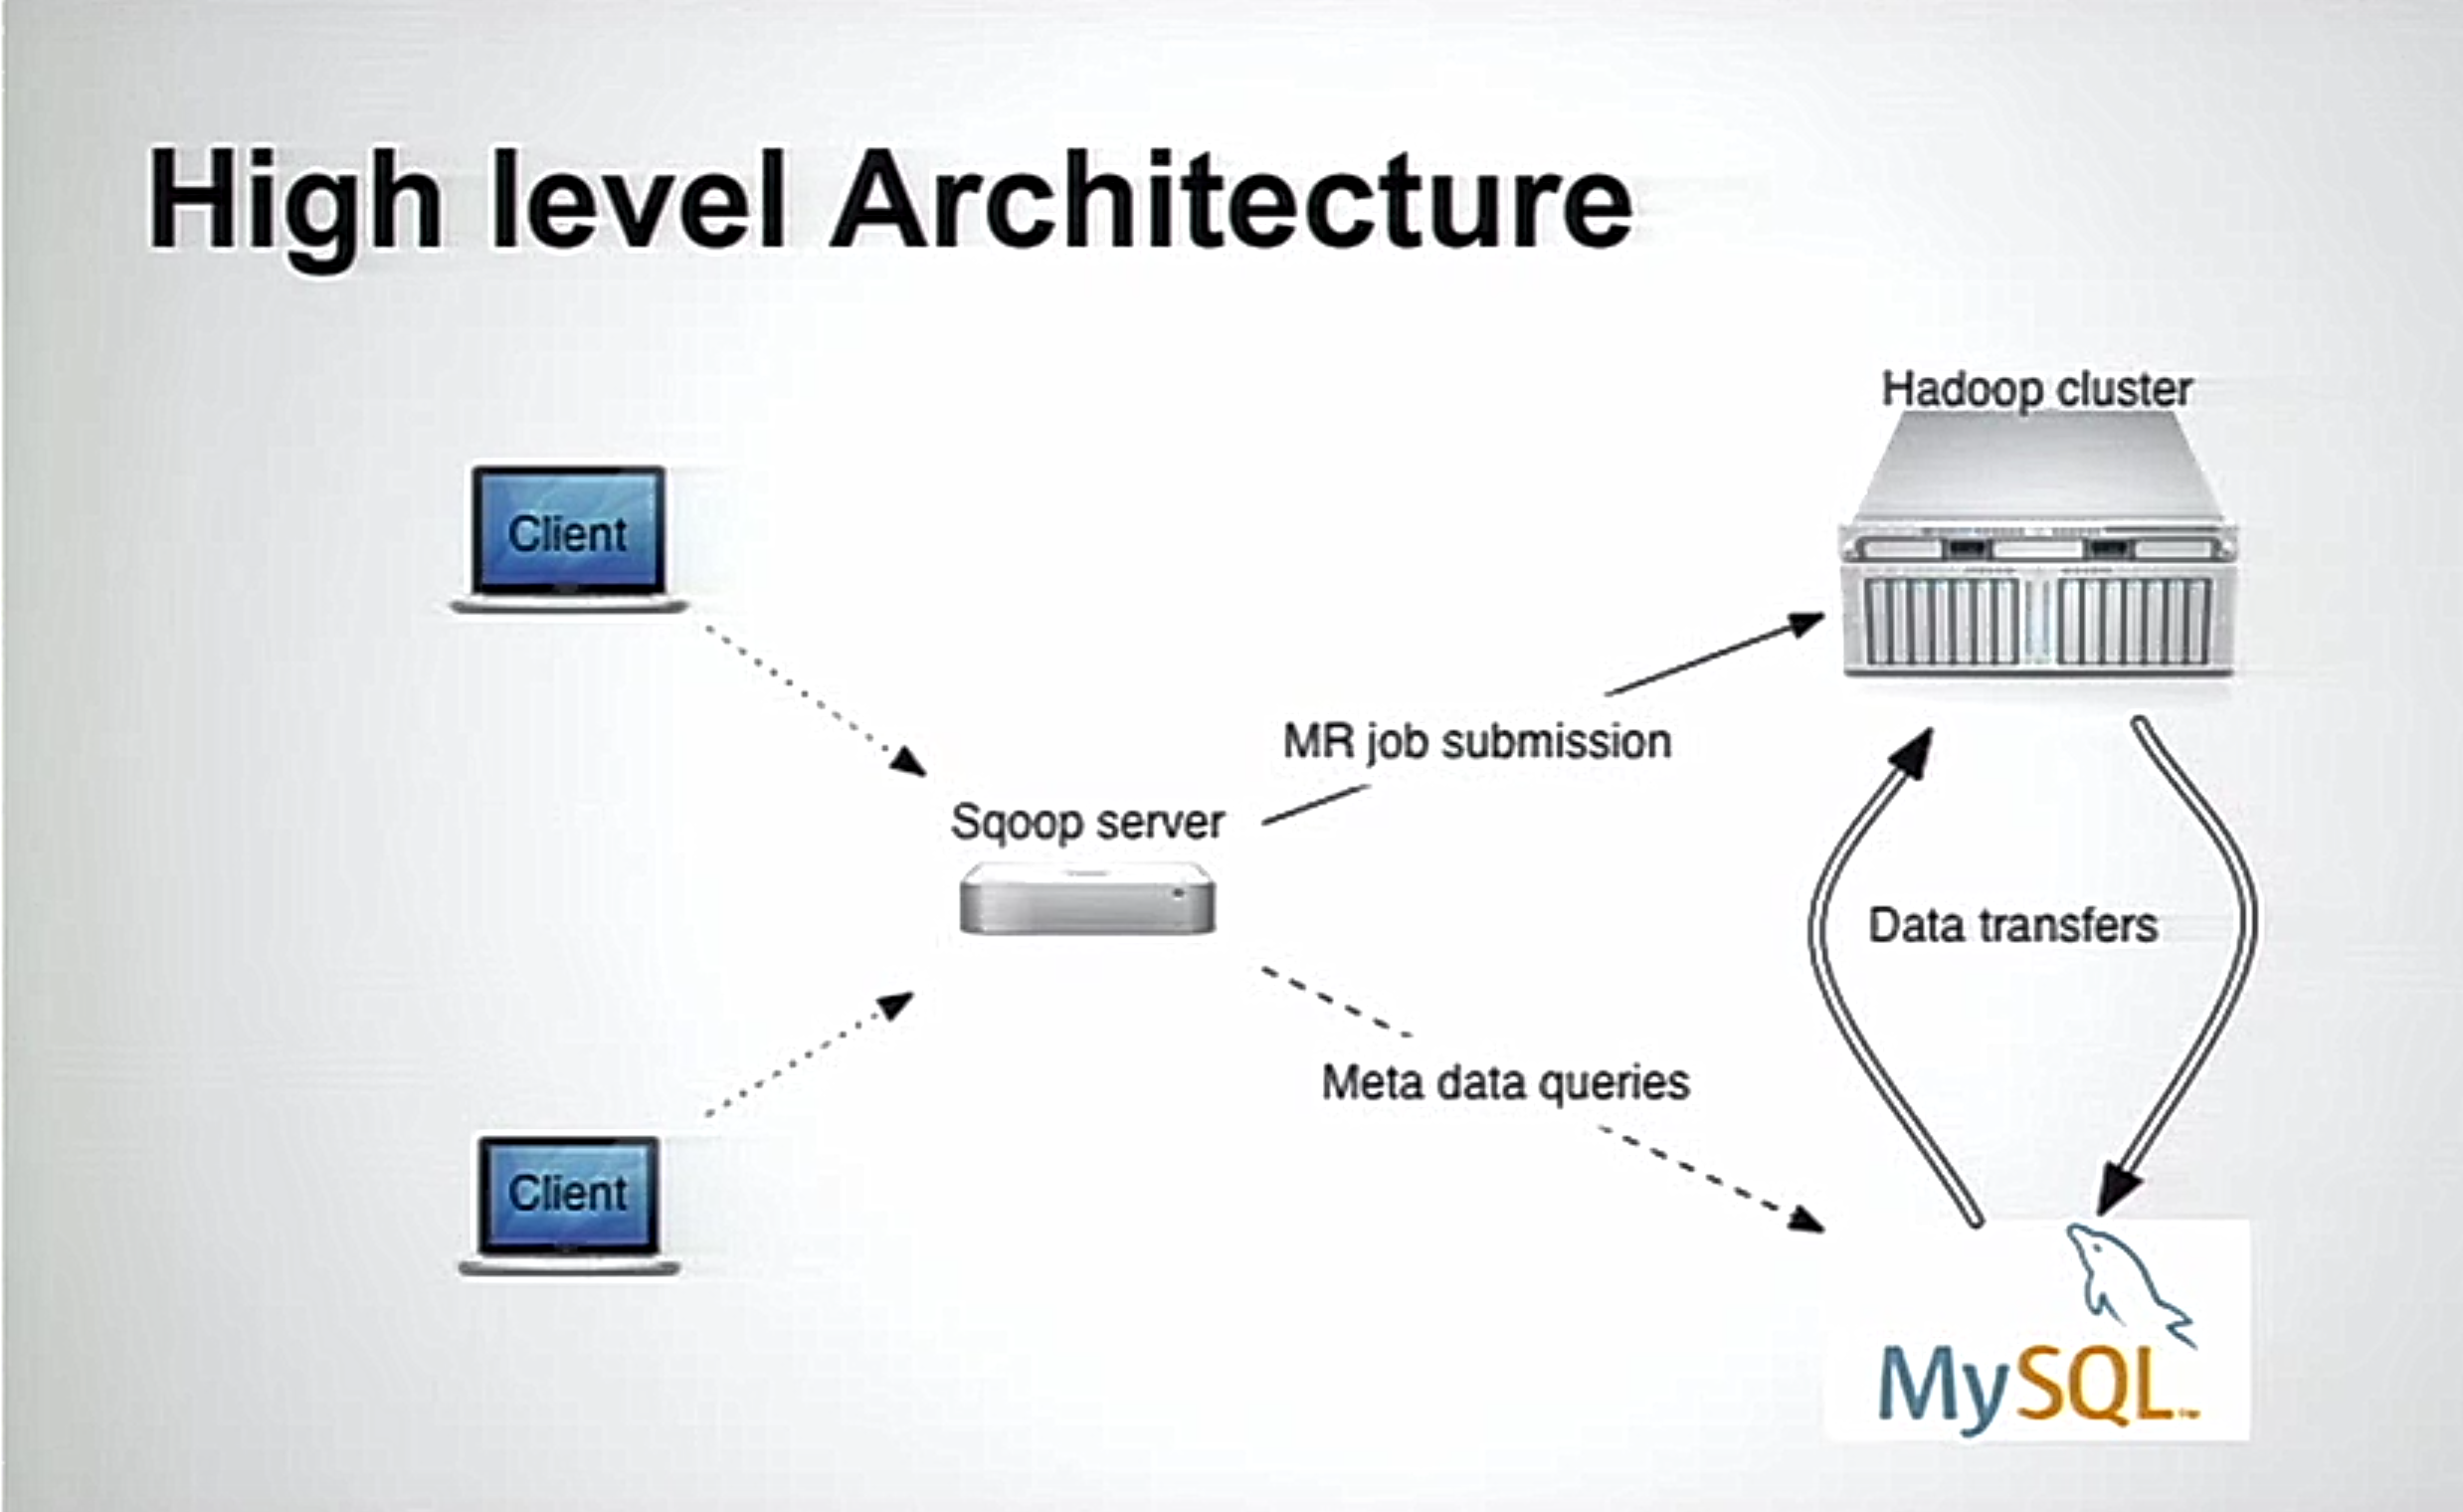
\includegraphics[width=\linewidth]{images/archi.png}
\caption{High Level Architecture of Sqoop \cite{sqoop-blog}}
\label{fig:archi}
\end{figure}


\section{Components of Sqoop}
\subsection{Connector}
Connectors are pluggable components that are used to communicate to RBDMS systems. There are pre defined connectors for many different type of databases, and there are generic JDBC connectors for any other new type of database. Connectors expose vital information like metadata to the Sqoop server. Connectors are responsible to move data in and out of RBDMs software. 
\subsection{Repository for Metadata}
Connectors fetch metadata information from each RDBMS servers and store them in repositories. This helps the work of Sqoop server in job management and to perform MapReduce on the requests.
\subsection{Server}
Servers have CRUD (create, read, update and delete) capabilities on the metadata repository. These capabilities are exposed via REST interface. Server also takes care of initiating data transfers. It is responsible for prioritising and managing the data transfer jobs. This also happens via REST interface. Sqoop server also monitors the jobs which are running to check their progress and failures. Sqoop server is independent of the actual data transfer and this is ideal for security purposes, since the actual data is not getting exposed. This also helps when Sqoop server is down for maintenance, the data transfers which are already in progress will continue to happen. 

\section{Workflow of Sqoop}
Figure \ref{fig:archi} shows the workflow of Sqoop. Sqoop server maintains the first two parts of the work flow -  initializing and partitioning the data transfer jobs. The next step is handled by connectors which extract data from RDBMS systems. This happens in parallel since the partitioner works on MapReduce algorithms to divide the job into parallel streams. The output is then sent to different nodes of Hadoop systems to load the data. The destroyer works to clean up all the temporary tables left behind by the entire process. The workflow resembles an ETL flow without the transformation phase.

\begin{figure}[htbp]
\centering
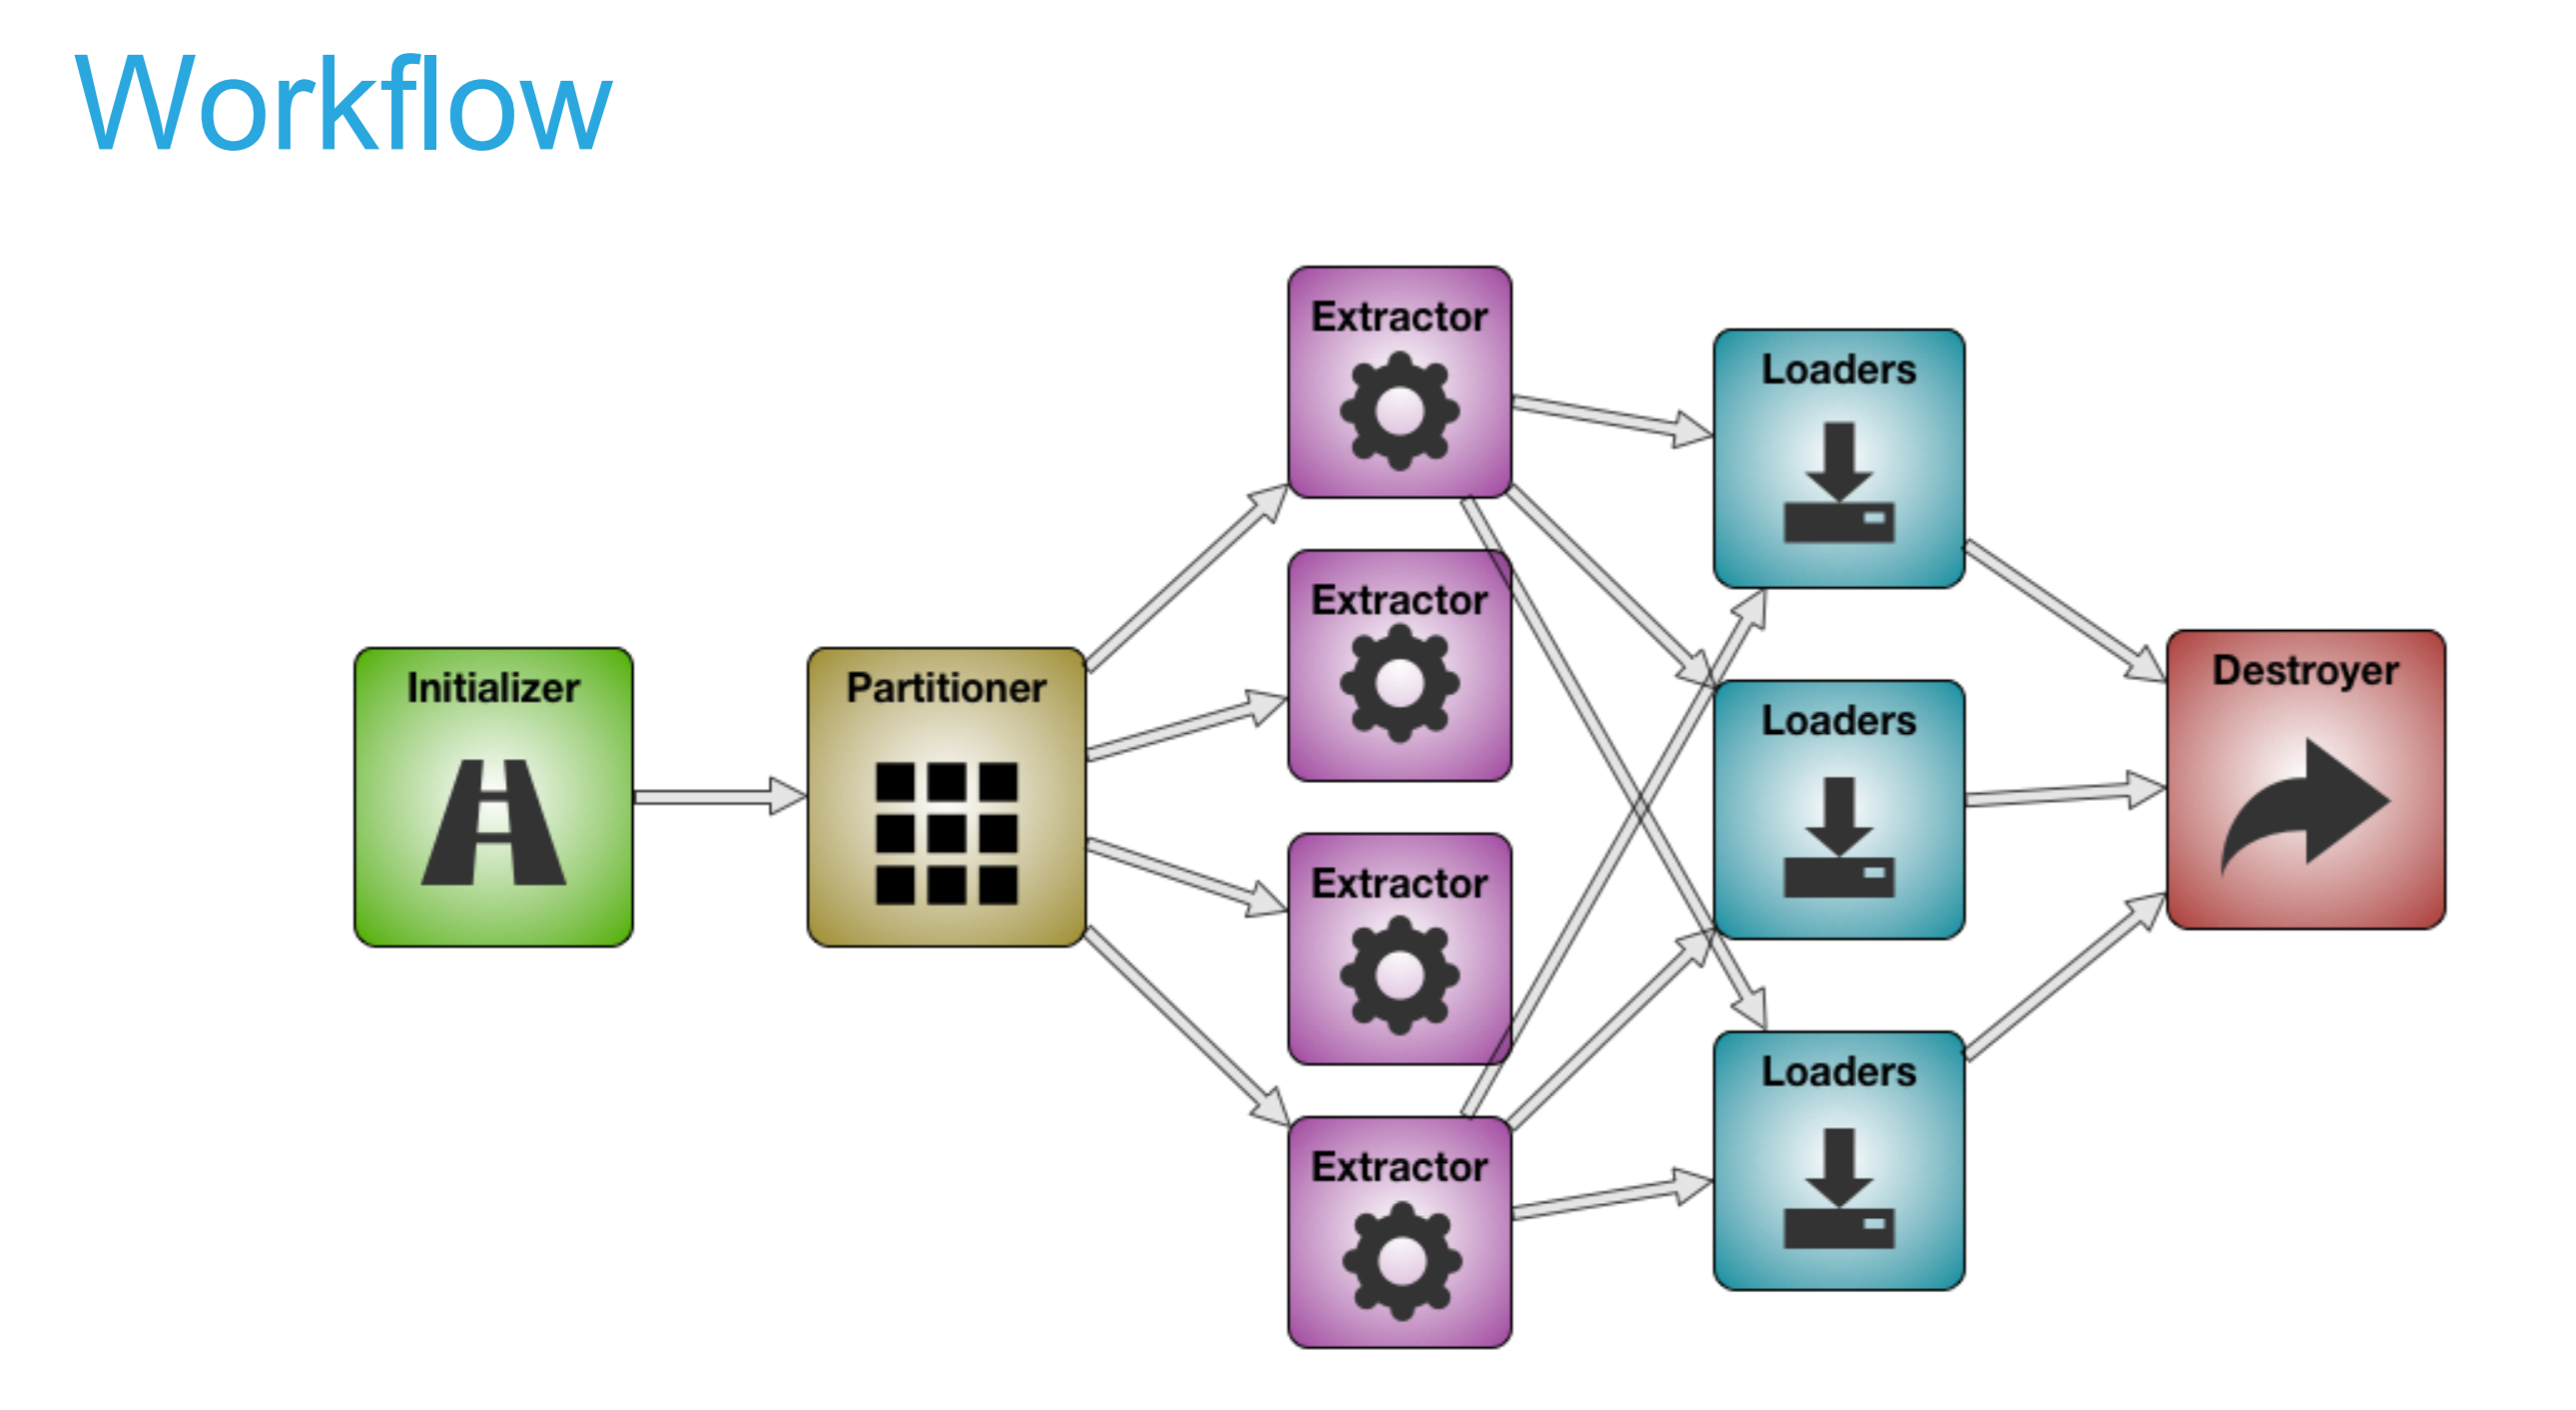
\includegraphics[width=\linewidth]{images/work.png}
\caption{Workflow Diagram \cite{sqoop-blog}}
\label{fig:work}
\end{figure}
\section{Licensing}
Apache Sqoop is available as an open source software, provided to download via multiple mirrors in the Sqoop website\cite{down}. The source code is also shared via GitHub \footnote{https://git-wip-us.apache.org/repos/asf?p=sqoop.git;a=summary} for developers to fork and modify it. 

\section{Shell Access}
The shell code for importing data from MYSQL, to Hive, HBase and exporting data is given in Algorithms 1, 2, 3 and 4\cite{cloudera}.

\begin{algorithm}
\caption{MYSQL Import}\label{alg:mysql}
\begin{quote}
\begin{Verbatim}[numbers=left]
sqoop import 
--connect jdbc:mysql://localhost/acmedb 
--table ORDERS 
--username test 
--password 
\end{Verbatim}
\end{quote}
\end{algorithm}
\begin{algorithm}
\caption{Hive Import}\label{alg:hive}
\begin{quote}
\begin{Verbatim}[numbers=left]
sqoop import 
--connect jdbc:mysql://localhost/acmedb 
--table ORDERS 
--username test 
--password
--hive-import
\end{Verbatim}
\end{quote}
\end{algorithm}
\begin{algorithm}
\caption{HBase Import}\label{alg:hbase}
\begin{quote}
\begin{Verbatim}[numbers=left]
sqoop import 
--connect jdbc:mysql://localhost/acmedb
--table ORDERS 
--username test 
--password 
--hbase-create-table 
--hbase-table ORDERS 
--column-family mysql
\end{Verbatim}
\end{quote}
\end{algorithm}

\begin{algorithm}
\caption{Export}\label{alg:export}
\begin{quote}
\begin{Verbatim}[numbers=left]
sqoop export
--connect jdbc:mysql://localhost/acmedb
--table ORDERS 
--username test 
--password **** 
--export-dir /user/asd
\end{Verbatim}
\end{quote}
\end{algorithm}

\section{Use Cases}
\subsection{Importing data into Hadoop}
One use case of Sqoop is to import data into Hadoop from MYSQL. In a typical banking scenario there can be a case where each users' transaction records are stored in a Hadoop system and the users' attributes can be stored in an RDBMS database. If we need to perform analyses into each users' transactions and link it to the users' attributes to check for fradulent transactions, we need to get the RDBMS data into the Hadoop system. Sqoop can be used to do this, by automatically pushing new updates in the RDBMS database into Hadoop. 

\subsection{Exporting data from Hadoop}
In the online search business, enormous amounts of data gets generated from user search queries, advertisements, clicks and views. In order to perform quick analyzes on the data like how many users clicked on a particular advertisement or how to price a particular slot, we need to aggregate the data from Hadoop and export it to RDBMS systems. 

\section{Conclusion}
Sqoop is an opensource software that helps to move efficiently data between RDBMS and Hadoop systems. In traditional systems we can get data dumps from ETL systems and push them to Hadoop using shell scripts. This process is time consuming to operate and develop. There are a lot of manual configurations involved like the file path and names. Sqoop can be used to avoid this hassles and automate and schedule these transfers easily. 

\section{Further Education}
Further learning about Sqoop is encouraged and informative materials can be found at the Apache Sqoop homepage\cite{pages}.

\section*{Acknowledgements}

The author thanks Professor Gregor Von Lazewski for providing us with the guidance and topics for the paper. The author also thanks the AIs of Big Data Class for providing the technical
support.


% Bibliography

\bibliography{references}
 
\section*{Author Biographies}
\begingroup
\setlength\intextsep{0pt}
\begin{minipage}[t][3.2cm][t]{1.0\columnwidth} % Adjust height [3.2cm] as required for separation of bio photos.
{\bfseries Harshit Krishnakumar} is pursuing his MSc in Data Science from
Indiana University Bloomington
\end{minipage}
\endgroup

\end{document}
